% !TeX TS-program = pdflatex


\documentclass[a4paper]{article}

% \usepackage[default]{fontsetup}

\usepackage{fancyhdr}
\usepackage{extramarks}
\usepackage{amsmath}
\usepackage{amsthm}
\usepackage{amsfonts}
\usepackage{tikz}
\usepackage[plain]{algorithm}
\usepackage{algpseudocode}
\usepackage{enumerate}
\usepackage{tikz}
\usepackage{tikz-qtree}
\usepackage{tikz-qtree-compat}
\usepackage{listings}


\lstset{
    basicstyle=\ttfamily,
	breaklines=true,
	framextopmargin=50pt,
	frame=bottomline,
	columns=fixed,       
    %numbers=left,                                       % 在左侧显示行号
	frame=none,                                          % 不显示背景边框
	backgroundcolor=\color[RGB]{255,255,255},            % 设定背景颜色
	keywordstyle=\color[RGB]{40,40,255},                 % 设定关键字颜色
	numberstyle=\footnotesize\color{darkgray},           % 设定行号格式
	commentstyle=\it\color[RGB]{0,96,96},                % 设置代码注释的格式
	stringstyle=\rmfamily\slshape\color[RGB]{128,0,0},   % 设置字符串格式
	showstringspaces=false,                              % 不显示字符串中的空格
	language=python,                                     % 设置语言
}
\usetikzlibrary{automata,positioning}

%
% Basic Document Settings
%  

\topmargin=-0.2in
\evensidemargin=0in
\oddsidemargin=0in
\textwidth=6.5in
\textheight=9.5in
\headsep=0.25in

\linespread{1.1}

\pagestyle{fancy}
\lhead{\hmwkAuthorName}
\chead{\hmwkClass : \hmwkTitle}
\rhead{\firstxmark}
\lfoot{\lastxmark}
\cfoot{\thepage}

\renewcommand\headrulewidth{0.4pt}
\renewcommand\footrulewidth{0.4pt}

\setlength\parindent{0pt}

%
% Create Problem Sections
%

\newcommand{\enterProblemHeader}[1]{
    \nobreak\extramarks{}{Problem \arabic{#1} continued on next page\ldots}\nobreak{}
    \nobreak\extramarks{Problem \arabic{#1} (continued)}{Problem \arabic{#1} continued on next page\ldots}\nobreak{}
}

\newcommand{\exitProblemHeader}[1]{
    \nobreak\extramarks{Problem \arabic{#1} (continued)}{Problem \arabic{#1} continued on next page\ldots}\nobreak{}
    \stepcounter{#1}
    \nobreak\extramarks{Problem \arabic{#1}}{}\nobreak{}
}

\newcommand*\circled[1]{\tikz[baseline=(char.base)]{
		\node[shape=circle,draw,inner sep=2pt] (char) {#1};}}


\setcounter{secnumdepth}{0}
\newcounter{partCounter}
\newcounter{homeworkProblemCounter}
\setcounter{homeworkProblemCounter}{1}
\nobreak\extramarks{Problem \arabic{homeworkProblemCounter}}{}\nobreak{}

%
% Homework Problem Environment
%
% This environment takes an optional argument. When given, it will adjust the
% problem counter. This is useful for when the problems given for your
% assignment aren't sequential. See the last 3 problems of this template for an
% example.
%

\newenvironment{homeworkProblem}[1][-1]{
    \ifnum#1>0
        \setcounter{homeworkProblemCounter}{#1}
    \fi
    \section{Problem \arabic{homeworkProblemCounter}}
    \setcounter{partCounter}{1}
    \enterProblemHeader{homeworkProblemCounter}
}{
    \exitProblemHeader{homeworkProblemCounter}
}

%
% Homework Details
%   - Title
%   - Class
%   - Due date
%   - Name
%   - Student ID

\newcommand{\hmwkTitle}{Homework\ \#01}
\newcommand{\hmwkClass}{Probability \& Statistics for EECS}
\newcommand{\hmwkDueDate}{2024-10-6}
\newcommand{\hmwkAuthorName}{Wenye Xiong}
\newcommand{\hmwkAuthorID}{2023533141}


%
% Title Page
%

\title{
    \vspace{2in}
    \textmd{\textbf{\hmwkClass:\\  \hmwkTitle}}\\
    \normalsize\vspace{0.1in}\small{Due\ on\ \hmwkDueDate\ at 23:59}\\
	\vspace{4in}
}

\author{
	Name: \textbf{\hmwkAuthorName} \\
	Student ID: \hmwkAuthorID}
\date{}

\renewcommand{\part}[1]{\textbf{\large Part \Alph{partCounter}}\stepcounter{partCounter}\\}

%
% Various Helper Commands
%

% Useful for algorithms
\newcommand{\alg}[1]{\textsc{\bfseries \footnotesize #1}}
% For derivatives
\newcommand{\deriv}[1]{\frac{\mathrm{d}}{\mathrm{d}x} (#1)}
% For partial derivatives
\newcommand{\pderiv}[2]{\frac{\partial}{\partial #1} (#2)}
% Integral dx
\newcommand{\dx}{\mathrm{d}x}
% Alias for the Solution section header
\newcommand{\solution}{\textbf{\large Solution}}
% Probability commands: Expectation, Variance, Covariance, Bias
\newcommand{\E}{\mathrm{E}}
\newcommand{\Var}{\mathrm{Var}}
\newcommand{\Cov}{\mathrm{Cov}}
\newcommand{\Bias}{\mathrm{Bias}}

\begin{document}


% \maketitle
% \thispagestyle{empty}
% \pagebreak

\date{
Due on Oct. 6, 2024, 23:59 UTC+8}
\title{SI 140A-02  Probability \& Statistics for EECS, Fall 2024 \\
Homework 1}
\maketitle
Read all the instructions below carefully before you start working on the assignment, and before you make a submission.
\begin{itemize}
    \item You are required to write down all the major steps towards making your conclusions; otherwise you may obtain limited points of the problem.
    \item Write your homework in English; otherwise you will get no points of this homework.
    \item Any form of plagiarism will lead to $0$ point of this homework. 
\end{itemize}
\newpage

\begin{homeworkProblem}[1]
\textbf{(Story Proof)} Define $\left\{\begin{array}{l}n \\ k\end{array}\right\}$ as the number of ways to partition $\{1,2, \ldots, n\}$ into $k$ non-empty subsets, or the number of ways to have $n$ students split up into $k$ groups such that each group has at least one student. For example, $\left\{\begin{array}{l}4 \\ 2\end{array}\right\}=7$ because we have the following possibilities:
$$
\begin{tabular}{ll}
$\bullet\{1\},\{2,3,4\}$ & $\bullet\{1,2\},\{3,4\}$ \\
$\bullet\{2\},\{1,3,4\}$ & $\bullet\{1,3\},\{2,4\}$ \\
$\bullet\{3\},\{1,2,4\}$ & $\bullet\{1,4\},\{2,3\}$ \\
$\bullet\{4\},\{1,2,3\}$ &
\end{tabular}
$$
Prove the following identities:\\
(a)
$$
\left\{\begin{array}{c}
n+1 \\
k
\end{array}\right\}=\left\{\begin{array}{c}
n \\
k-1
\end{array}\right\}+k\left\{\begin{array}{l}
n \\
k
\end{array}\right\} .
$$
Hint: I'm either in a group by myself or I'm not.\\
(b)
$$
\sum_{j=k}^n\left(\begin{array}{l}
n \\
j
\end{array}\right)\left\{\begin{array}{l}
j \\
k
\end{array}\right\}=\left\{\begin{array}{l}
n+1 \\
k+1
\end{array}\right\} .
$$
Hint: First decide how many people are not going to be in my group.


\subsection{Solution}
(a)\\
\textbf{Proof:} \\
Consider the number of ways to have $n+1$ students split up into $k$ groups.
We consider the following two cases:
\begin{itemize}
    \item Case 1: I'm in a group by myself.\\
    In this case, we have $n$ students and $k-1$ groups. The number of ways to partition the remaining $n$ students into $k-1$ groups is $\left\{\begin{array}{c}
n \\
k-1
\end{array}\right\}$.
    \item Case 2: I'm not in a group by myself.\\
    In this case, we first pretend I doesn't exist and consider that we have $n$ students and $k$ groups. The number of ways to partition the $n$ students into $k$ groups is $\left\{\begin{array}{l}
n \\
k
\end{array}\right\}$.\\
    Then for each of the k groups, I can choose to join a random group. So there are $k\left\{\begin{array}{l}
n \\
k
\end{array}\right\}$ ways to partition the $n$ students into $k$ groups.
\end{itemize}
Therefore, we have
$$
\left\{\begin{array}{c}
n+1 \\
k
\end{array}\right\}=\left\{\begin{array}{c}
n \\
k-1
\end{array}\right\}+k\left\{\begin{array}{l}
n \\
k
\end{array}\right\} .
$$
\newpage
(b)\\
\textbf{Proof:} \\
Consider the number of ways to have $n+1$ students split up into $k+1$ groups. According to the definition, this number is $\left\{\begin{array}{l}
n+1 \\
k+1
\end{array}\right\}$.
We then consider if there are $j$ students not going to be in my group, where $j$ ranges from $k$ to $n$ such that no group is empty.
For each $j$, the number of ways to partition the $n+1$ students into $j$ is $\left(\begin{array}{l}
n \\
j
\end{array}\right)$, and the number of ways to partition the $j$ students into $k$ groups is $\left\{\begin{array}{l}
j \\
k
\end{array}\right\}$.
Therefore, the total number of ways to partition the $n+1$ students into $k+1$ groups is
$$
\sum_{j=k}^n\left(\begin{array}{l}
n \\
j
\end{array}\right)\left\{\begin{array}{l}
j \\
k
\end{array}\right\}
$$
Thus we have proved that 
$$
\sum_{j=k}^n\left(\begin{array}{l}
n \\
j
\end{array}\right)\left\{\begin{array}{l}
j \\
k
\end{array}\right\}=\left\{\begin{array}{l}
n+1 \\
k+1
\end{array}\right\} .
$$
\end{homeworkProblem}


\newpage
\begin{homeworkProblem}[2]
A \textit{norepeatword} is a sequence of at least one (and possibly all) of the usual 26 letters a, b, c, .., z, with repetitions not allowed. For example, "course" is a norepeatword, but "statistics" is not. Order matters, e.g., "course" is not the same as "source". A norepeatword is chosen randomly, with all norepeatwords equally likely. Show that the probability that it uses all 26 letters is very close to $1 / e$.

\subsection{Solution}
\textbf{Proof:} \\
The number of norepeatwords that use all 26 letters is the number of ordered arrangements of 26 letters, which is $26!$. The total number of norepeatwords is the sum of the number of norepeatwords that use $k$ letters for $1 \leq k \leq 26$. To calculate the number of norepeatword with $k$ letters, we first choose $k$ letters from the 26 letters, which can be done in $\left(\begin{array}{l}26 \\ k\end{array}\right)$ ways. Then we arrange the $k$ letters in $k!$ ways. Therefore, the number of norepeatwords with $k$ letters is $\left(\begin{array}{l}26 \\ k\end{array}\right) k!$.\\
Thus the total number of norepeatwords is
$$
\sum_{k=1}^{26}\left(\begin{array}{l}26 \\ k\end{array}\right) k!.
$$
And the probability that a norepeatword uses all 26 letters is
$$
\frac{26 !}{\sum_{k=1}^{26}\left(\begin{array}{l}26 \\ k\end{array}\right) k !}=\frac{26 !}{\sum_{k=1}^{26} \frac{26 !}{k ! (26-k) !} k !} .\\
= \frac{1}{\sum_{k=1}^{26} \frac{1}{(26-k) !}}=\frac{1}{\sum_{k=0}^{25} \frac{1}{k !}}.
$$
According to the Taylor series expansion of $e$, we have
$$
e=\sum_{k=0}^{\infty} \frac{1}{k !} .
$$
And the denominator of the probability is exactly the sum of the first 26 terms of the Taylor series expansion of $e$. Therefore, the probability that a norepeatword uses all 26 letters is very close to $1 / e$.
\end{homeworkProblem}



\newpage
\begin{homeworkProblem}[3]
Given $n \geq 2$ numbers $\left(a_1, a_2, \ldots, a_n\right)$ with no repetitions, a bootstrap sample is a sequence $\left(x_1, x_2, \ldots, x_n\right)$ formed from the $a_j$ 's by sampling with replacement with equal probabilities. Bootstrap samples arise in a widely used statistical method known as the bootstrap. For example, if $n=2$ and $\left(a_1, a_2\right)=(3,1)$, then the possible bootstrap samples are $(3,3),(3,1),(1,3)$, and $(1,1)$.\\
(a) How many possible bootstrap samples are there for $\left(a_1, \ldots, a_n\right)$ ?\\
(b) How many possible bootstrap samples are there for $\left(a_1, \ldots, a_n\right)$, if order does not matter (in the sense that it only matters how many times each $a_j$ was chosen, not the order in which they were chosen)?\\
(c) One random bootstrap sample is chosen (by sampling from $a_1, \ldots, a_n$ with replacement, as described above). Show that not all unordered bootstrap samples (in the sense of (b)) are equally likely. Find an unordered bootstrap sample $\mathbf{b}_1$ that is as likely as possible, and an unordered bootstrap sample $\mathbf{b}_2$ that is as unlikely as possible. Let $p_1$ be the probability of getting $\mathbf{b}_1$ and $p_2$ be the probability of getting $\mathbf{b}_2$ (so $p_i$ is the probability of getting the specific unordered bootstrap sample $\mathbf{b}_i$ ). What is $p_1 / p_2$ ? What is the ratio of the probability of getting an unordered bootstrap sample whose probability is $p_1$ to the probability of getting an unordered sample whose probability is $p_2$ ?

\subsection{Solution}
(a)\\
Consider the number of ways to choose $n$ numbers from $n$ numbers with replacement. For each number, there are $n$ choices. Therefore, the total number of possible bootstrap samples is $n^n$.\\
(b)\\
If order does not matter, then the number of possible bootstrap samples is the number of ways to partition $n$ objects into $n$ subsets (empty subset allowed), which is $\left(\begin{array}{l}2n-1 \\ n-1\end{array}\right)$ according to the conclusion of Bose-Einstein Problem.\\
(c)\\
Consider a specific unordered bootstrap sample $\mathbf{s}$  $(s_1, s_2, \ldots, s_n)$, where $s_i$ is the number of times $a_i$ is chosen. The total number of way to get $\mathbf{s}$ is
$$
\frac{n !}{s_1 ! s_2 ! \cdots s_n !}.
$$
This is because there are $n!$ ways to arrange the $n$ numbers, but we need to divide by $s_1!$ for the $s_1$ times $a_1$ is chosen, $s_2!$ for the $s_2$ times $a_2$ is chosen, and so on.\\
Thus the probability of getting $\mathbf{s}$ is
$$
\frac{1}{n^n} \frac{n !}{s_1 ! s_2 ! \cdots s_n !}=\frac{n!}{s_1 ! s_2 ! \cdots s_n ! n^n}.
$$
Both $n!$ and $n^n$ are constant, so the probability of getting $\mathbf{s}$ is proportional to $\frac{1}{s_1 ! s_2 ! \cdots s_n !}$. To find the unordered bootstrap sample $\mathbf{b}_1$ that is as likely as possible, we need to find the $\mathbf{s}$ that minimizes $s_1 ! s_2 ! \cdots s_n !$. Since the sum of the $s_i$ is $n$, the minimum value of $s_1 ! s_2 ! \cdots s_n !$ is achieved when all $s_i$ equal to 1. And the probability of getting $\mathbf{b}_1$ is
$$
p_1 = \frac{n !}{1 ! 1 ! \cdots 1 ! n^n}=\frac{n!}{n ^n}.
$$
Similarly, to find the unordered bootstrap sample $\mathbf{b}_2$ that is as unlikely as possible, we need to find the $\mathbf{s}$ that maximizes $s_1 ! s_2 ! \cdots s_n !$. That is when $s_1=n$ and $s_i=0$ for $i \neq 1$. The probability of getting $\mathbf{b}_2$ is
$$
p_2 = \frac{n !}{n ! 0 ! \cdots 0 ! n^n}=\frac{n!}{n! n^n}=\frac{1}{n^n}.
$$
Therefore, $p_1 / p_2 = n!$. \\
But the ratio of the probability of getting an unordered bootstrap sample whose probability is $p_1$ to the probability of getting an unordered sample whose probability is $p_2$ is different from that: $\mathbf{b}_1 = (1,1,\cdots,1)$ is the only unordered bootstrap sample whose probability is $p_1$. However, there are n unordered bootstrap samples whose probability is $p_2$, which are $(n,0,\cdots,0)$, $(0,n,0,\cdots,0)$, $\cdots$, $(0,0,\cdots,n)$. Therefore, the ratio is 
$$
\frac{n!}{n} = (n-1)!.
$$
\end{homeworkProblem}

\newpage
\begin{homeworkProblem}[4]
\textbf{(Geometric Probability)} You get a stick and break it randomly into three pieces. What is the probability that you can make a triangle using such three pieces?
\subsection{Solution}
Assume the stick has length l, and the first and second pieces have length $x$ and $y$, respectively. Then the third piece has length $l-x-y$. To form a triangle, the sum of the lengths of any two pieces must be greater than the length of the third piece. Therefore, we have the following three inequalities:
$$
\begin{aligned}
x+y &> l-x-y, \\
x+(l-x-y) &> y, \\
y+(l-x-y) &> x.
\end{aligned}
$$
Solving these inequalities, we have
$$
\begin{aligned}
x &< \frac{l}{2}, \\
y &< \frac{l}{2}, \\
x + y &> \frac{l}{2}.
\end{aligned}
$$
To solve the probability, we can use Geometric Probability and draw a diagram to help us. We first draw a two dimensional coordinate system with the x-axis representing the length of the first piece and the y-axis representing the length of the second piece. 
The region that satisfies three pieces broken from a stick with length l is a triangle with vertices $(0,0),(l,0),(0,l)$. 
The region that satisfies the three inequalities is another triangle inside it with vertices $(0,\frac{l}{2}),(\frac{l}{2},0),(\frac{l}{2},\frac{l}{2})$.
Therefore, the probability that you can make a triangle using such three pieces is the ratio of the area of the smaller triangle to the area of the larger triangle, which is $\frac{1}{4}$.
Here's the diagram:
\begin{center}
    \begin{tikzpicture}
        \draw[->] (0,0) -- (5,0) node[right] {$x$};
        \draw[->] (0,0) -- (0,5) node[above] {$y$};
        \draw (0,0) -- (4,0) -- (0,4) -- cycle;
        \draw[dashed] (0,2) -- (2,0) -- (2,2) -- cycle;
        \node[below] at (2,0) {$\frac{l}{2}$};
        \node[left] at (0,2) {$\frac{l}{2}$};
        \node[left] at (0,4) {$l$};
        \node[below] at (4,0) {$l$};
        \node[above right] at (2,2) {$\left(\frac{l}{2},\frac{l}{2}\right)$};
    \end{tikzpicture}
\end{center}

\end{homeworkProblem}

\newpage
\begin{homeworkProblem}[5]
In the birthday problem, we assumed that all 365 days of the year are equally likely (and excluded February 29). In reality, some days are slightly more likely as birthdays than others. For example, scientists have long struggled to understand why more babies are born 9 months after a holiday. Let $\mathbf{p}=\left(p_1, p_2, \ldots, p_{365}\right)$ be the vector of birthday probabilities, with $p_j$ the probability of being born on the $j$ th day of the year (February 29 is still excluded, with no offense intended to Leap Dayers). The $k$ th elementary symmetric polynomial in the variables $x_1, \ldots, x_n$ is defined by
$$
e_k\left(x_1, \ldots, x_n\right)=\sum_{1 \leq j_1<j_2<\cdots<j_k \leq n} x_{j_1} \ldots x_{j_k} .
$$
This just says to add up all of the $\left(\begin{array}{l}n \\ k\end{array}\right)$ terms we can get by choosing and multiplying $k$ of the variables. For example, $e_1\left(x_1, x_2, x_3\right)=x_1+x_2+x_3, e_2\left(x_1, x_2, x_3\right)=x_1 x_2+$ $x_1 x_3+x_2 x_3$, and $e_3\left(x_1, x_2, x_3\right)=x_1 x_2 x_3$ Now let $k \geq 2$ be the number of people.\\
(a) Find a simple expression for the probability that there is at least one birthday match, in terms of $\mathbf{p}$ and an elementary symmetric polynomial.\\
(b) Explain intuitively why it makes sense that $P$ (at least one birthday match) is minimized when $p_j=\frac{1}{365}$ for all $j$, by considering simple and extreme cases.\\
(c) The famous arithmetic mean-geometric mean inequality says that for $x, y \geq 0$
$$
\frac{x+y}{2} \geq \sqrt{x y} .
$$
This inequality follows from adding $4 x y$ to both sides of $x^2-2 x y+y^2=(x-y)^2 \geq 0$ Define $\mathbf{r}=\left(r_1, \ldots, r_{365}\right)$ by $r_1=r_2=\left(p_1+p_2\right) / 2, r_j=p_j$ for $3 \leq j \leq 365$. Using the arithmetic mean-geometric mean bound and the fact, which you should verify, that
$$
e_k\left(x_1, \ldots, x_n\right)=x_1 x_2 e_{k-2}\left(x_3, \ldots, x_n\right)+\left(x_1+x_2\right) e_{k-1}\left(x_3, \ldots, x_n\right)+e_k\left(x_3, \ldots, x_n\right)
$$
show that

\begin{center}
    $P($ at least one birthday match $\mid \mathbf{p}) \geq P($ at least one birthday match $\mid \mathbf{r})$
\end{center}

% \vspace{8pt}
with strict inequality if $\mathbf{p} \neq \mathbf{r}$, where the given $\mathbf{r}$ notation means that the birthday probabilities are given by $\mathbf{r}$. Using this, show that the value of $\mathbf{p}$ that minimizes the probability of at least one birthday match is given by $p_j=\frac{1}{365}$ for all $j$.

\subsection{Solution}
(a)\\
$1 - k!e_{k}\left(\overrightarrow{p}\right)$ is the probability that there is at least one birthday match.\\
\textbf{Proof:} \\
The probability that there is at least one birthday match is $1$ minus the probability that there is no birthday match. The probability that there is no birthday match is the probability that all $k$ people have different birthdays, which is the number of ways to partition $k$ people into $k$ subsets (each subset represents a birthday) times the probability that each person has a different birthday. The number of ways to partition $k$ people into $k$ subsets is $k!$, and the probability that each person has a different birthday is $e_{k}\left(\overrightarrow{p}\right)$. Therefore, the probability that there is at least one birthday match is $1 - k!e_{k}\left(\overrightarrow{p}\right)$.\\
(b)\\
Consider a simple but extreme case where $p_{1} = 1$ and $p_{i} = 0$ for $i \neq 1$. 
Then, the probability that there is at least one birthday match is $1$ since all k people are born in the same day. 
But if we change $p_{i}$ to $\frac{1}{365}$ for all i, then the probability that there is at least one birthday match is a number less than 1.
In general, if $p_{i} > \frac{1}{365}$ for a particular $i$, then a birthday match is more likely to happen, since the probability that a person is born on that day is higher.
Thus, it makes intuitive sense that the probability of at least one birthday match is minimized when $p_{i} = \frac{1}{365}$.\\
(c)\\
\textbf{Proof:} \\
First we verify the fact that
$$
e_k\left(x_1, \ldots, x_n\right)=x_1 x_2 e_{k-2}\left(x_3, \ldots, x_n\right)+\left(x_1+x_2\right) e_{k-1}\left(x_3, \ldots, x_n\right)+e_k\left(x_3, \ldots, x_n\right).
$$
The proof is as follows:
\begin{itemize}
    \item If $x_1$ and $x_2$ are not chosen, then the number of ways to partition the remaining $n$ variables into $k$ subsets is $e_k\left(x_3, \ldots, x_n\right)$.
    \item If $x_1$ is chosen but $x_2$ is not chosen, then the number of ways to partition the remaining $n$ variables into $k$ subsets is $x_1 e_{k-1}\left(x_3, \ldots, x_n\right)$. And this is the same as the number of ways to partition the remaining $n$ variables into $k$ subsets if $x_2$ is chosen but $x_1$ is not chosen, which is $x_2 e_{k-1}\left(x_3, \ldots, x_n\right)$.
    \item If $x_1$ and $x_2$ are both chosen, then the number of ways to partition the remaining $n$ variables into $k$ subsets is $x_1 x_2 e_{k-2}\left(x_3, \ldots, x_n\right)$.
    \item Therefore, the total number of ways to partition the $n$ variables into $k$ subsets is $x_1 x_2 e_{k-2}\left(x_3, \ldots, x_n\right)+\left(x_1+x_2\right) e_{k-1}\left(x_3, \ldots, x_n\right)+e_k\left(x_3, \ldots, x_n\right)$.
    \item Thus we have verified the fact.
\end{itemize}
Now we consider $e_k\left(\overrightarrow{p}\right)$ and $e_k\left(\overrightarrow{r}\right)$: After expansion of $e_k\left(\overrightarrow{p}\right)$ and $e_k\left(\overrightarrow{r}\right)$, we have
$$
\begin{aligned}
e_k\left(\overrightarrow{p}\right) &= p_1 p_2 e_{k-2}\left(p_3, \ldots, p_{365}\right)+\left(p_1+p_2\right) e_{k-1}\left(p_3, \ldots, p_{365}\right)+e_k\left(p_3, \ldots, p_{365}\right), \\
e_k\left(\overrightarrow{r}\right) &= r_1 r_2 e_{k-2}\left(r_3, \ldots, r_{365}\right)+\left(r_1+r_2\right) e_{k-1}\left(r_3, \ldots, r_{365}\right)+e_k\left(r_3, \ldots, r_{365}\right).
\end{aligned}
$$
Since $r_1 = r_2 = \frac{p_1+p_2}{2}$, and $r_j = p_j$ for $3 \leq j \leq 365$, we can easily find that the only difference between
$e_k\left(\overrightarrow{p}\right)$ and $e_k\left(\overrightarrow{r}\right)$ is the terms $p_1 p_2 e_{k-2}\left(p_3, \ldots, p_{365}\right)$ and $r_1 r_2 e_{k-2}\left(r_3, \ldots, r_{365}\right)$. 
According to the arithmetic mean-geometric mean inequality, we have
$$
\frac{p_1+p_2}{2} \geq \sqrt{p_1 p_2}.
$$
Therefore, we have
$$
r_1 r_2 e_{k-2}\left(r_3, \ldots, r_{365}\right) \geq p_1 p_2 e_{k-2}\left(p_3, \ldots, p_{365}\right).
$$
Thus we have
$$
e_k\left(\overrightarrow{p}\right) \leq e_k\left(\overrightarrow{r}\right).
$$
And the strict inequality holds if $\overrightarrow{p} \neq \overrightarrow{r}$.\\
According to the conclusion of (a), $P($ at least one birthday match $\mid \overrightarrow{p}) = 1 - k!e_{k}\left(\overrightarrow{p}\right)$, and $P($ at least one birthday match $\mid \overrightarrow{r}) = 1 - k!e_{k}\left(\overrightarrow{r}\right)$. 
Therefore, we have shown that $P($ at least one birthday match $\mid \overrightarrow{p}) \geq P($ at least one birthday match $\mid \overrightarrow{r})$ with strict inequality if $\overrightarrow{p} \neq \overrightarrow{r}$.\\
Next, to prove that the value of $\overrightarrow{p}$ that minimizes the probability of at least one birthday match is given by $p_j=\frac{1}{365}$ for all $j$, we consider the case where 
some of the $p_j$ are not equal to $\frac{1}{365}$. Suppose that the value of $\overrightarrow{p}$ that minimizes the probability of at least one birthday match is $\overrightarrow{p} = \overrightarrow{p'}$ where $p'_j \neq \frac{1}{365}$ for some $j$. 
With the conclusion above, we find that we can take out any two $p'_j \neq \frac{1}{365}$ and replace them with their average, which will decrease the probability of at least one birthday match.
This contradicts the assumption that $\overrightarrow{p'}$ minimizes the probability of at least one birthday match.
Therefore, the value of $\overrightarrow{p}$ that minimizes the probability of at least one birthday match is given by $p_j=\frac{1}{365}$ for all $j$ since taking average of any two $p_j = \frac{1}{365}$ will contribute to nothing.\\
\end{homeworkProblem}

\newpage
\begin{homeworkProblem}[6]
\textbf{(Coupon Collection)} If each box of a brand of crispy instant noodle contains a coupon, and there are 108 different types of coupons. Given $n \geq 200$, what is the probability that buying $n$ boxes can collect all 108 types of coupons? You also need to plot a figure to show how such probability changes with the increasing value of $n$. When such probability is no less than $95 \%$, what is the minimum number of $n$ ?
\subsection{Solution}
There are 108 different types of coupons in total. So for the n boxes, there are exactly $108^n$ possible outcomes. 
If we want to solve out the probability that buying $n$ boxes can collect all 108 types of coupons, we just need to calculate the number of ways to satisfy the condition that all 108 types of coupons are collected and divide it by $108^n$.\\
The number of ways to collect all 108 types of coupons is the number of ways to partition $n$ different boxes into 108 different non-empty subsets (each subset represents a type of coupon).\\
In Problem 1, we defined the number of ways to partition $n$ different objects into $k$ non-empty subsets as $\left\{\begin{array}{c}n \\ k\end{array}\right\}$.
Easily, we can find that the number of ways to partition $n$ different boxes into 108 different non-empty subsets is $ k! \left\{\begin{array}{c}n \\ 108\end{array}\right\}$, since the order of the 108 types of coupons matters.\\
Therefore, the probability that buying $n$ boxes can collect all 108 types of coupons is
$$
\frac{108! \left\{\begin{array}{c}n \\ 108\end{array}\right\}}{108^n}.
$$
To find the minimum number of $n$ when such probability is no less than $95 \%$, we need to solve the following inequality:
$$
\frac{108! \left\{\begin{array}{c}n \\ 108\end{array}\right\}}{108^n} \geq 0.95.
$$
From last semester's Discrete Math course, I learned that $\left\{\begin{array}{c}n \\ k\end{array}\right\} $ is actually the Stirling number of the second kind, which can be solved with the following formula:
$$
\left\{\begin{array}{c}n \\ k\end{array}\right\} = \frac{1}{k!} \sum_{j=0}^{k} (-1)^{k-j} \left(\begin{array}{c}k \\ j\end{array}\right) j^n.
$$
This can be proved by the principle of inclusion-exclusion: the number of ways to partition $n$ different objects into $k$ non-empty subsets is the number of ways to partition $n$ different objects into $k$ subsets minus the number of ways to partition $n$ different objects into $k-1$ subsets, plus the number of ways to partition $n$ different objects into $k-2$ subsets, and so on.\\
However, in actual programming, this formula is still too difficult to calculate. So I decided to use the Monte Carlo method to simulate the process of buying $n$ boxes and collecting all 108 types of coupons. The code is as follows:
\begin{lstlisting}
    import random
    import numpy as np
    import matplotlib.pyplot as plt

    def simulate_coupon_collection(n, m, iterations=1000):
        success_count = 0
        for i in range(iterations):
            collected_coupons = set()
            for j in range(n):
                coupon = random.randint(1, m)
                collected_coupons.add(coupon)
            if len(collected_coupons) == m:
                success_count += 1

        probability = (success_count / iterations) * 100
        return probability

    # Parameters
    m = 108  # Number of coupon types
    iterations = 1000  # Number of simulation iterations

    # Run the simulation
    target = 0
    for n in range(200, 1000, 10):
        probability = simulate_coupon_collection(n, m, iterations)
        if probability >= 95 and target == 0:
            target = n
        print(f"Probability of collecting all {m} coupons after {n} trials: {probability:.2f}%")
        plt.scatter(n, probability, color='blue')
    plt.axhline(y=95, color='r', linestyle='-')
    plt.xlabel("Number of Trials")
    plt.ylabel("Probability (%)")
    plt.title("Coupon Collection Simulation")
    plt.text(200, 95, f"First reach probability 95%: {target}", color='red')
    plt.show()
\end{lstlisting}
The plot is as follows:
\begin{center}
    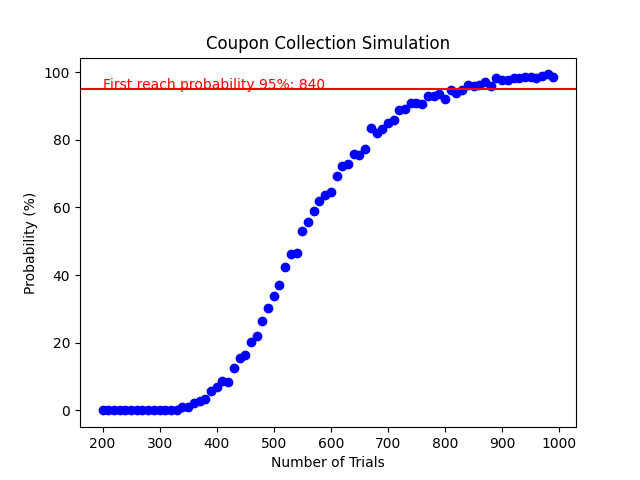
\includegraphics[width=0.8\textwidth]{Coupon Collection Simulation.png}
\end{center}
From the plot, we can see that the probability of collecting all 108 coupons increases with the number of trials. When the number of trials is around 840, the probability reaches 95\%. 
Note that this is just a simple and rough simulation. The actual number of trials may be different due to the randomness of the simulation. But according to the plot, we can conclude that the minimum number of $n$ when such probability is no less than $95 \%$ is around 840.

\end{homeworkProblem}





\end{document}
